\documentclass[aspectratio=169]{beamer}

\mode<presentation>

\usepackage[utf8]{inputenc}
\usepackage[T1]{fontenc}	%makes å,ä,ö etc. proper symbols
\usepackage{amsmath}
\usepackage{graphicx}
\usepackage{xcolor}
\usepackage{listings}
\usepackage{multicol}
\usepackage{multirow}
\usepackage{hyperref}
\usepackage[swedish]{babel}

\definecolor{LundaGroen}{RGB}{00,68,71}
\definecolor{StabilaLila}{RGB}{85,19,78}
\definecolor{VarmOrange}{RGB}{237,104,63}

\definecolor{MagnoliaRosa}{RGB}{251,214,209}
\definecolor{LundaHimmel}{RGB}{204,225,225}
\definecolor{LundaLjus}{RGB}{255,242,191}

\usefonttheme{serif}
\usetheme{malmoe}
\setbeamercolor{palette primary}{bg=LundaHimmel, fg=StabilaLila}
\setbeamercolor{palette quaternary}{bg=LundaGroen, fg=MagnoliaRosa}
\setbeamercolor{background canvas}{bg=LundaLjus}
\setbeamercolor{structure}{fg=LundaGroen}

\usepackage[many]{tcolorbox}

\newtcolorbox{cross}{blank,breakable,parbox=false,
  overlay={\draw[red,line width=5pt] (interior.south west)--(interior.north east);
    \draw[red,line width=5pt] (interior.north west)--(interior.south east);}}
    
\newcommand{\code}[1]{\colorbox{white}{\lstinline{#1}}}



\lstset{language=Python} 
\lstset{%language=[LaTeX]Tex,%C++,
    morekeywords={PassOptionsToPackage,selectlanguage,True,False},
    keywordstyle=\color{blue},%\bfseries,
    basicstyle=\small\ttfamily,
    %identifierstyle=\color{NavyBlue},
    commentstyle=\color{red}\ttfamily,
    stringstyle=\color{VarmOrange},
    numbers=left,%
    numberstyle=\scriptsize,%\tiny
    stepnumber=1,
    numbersep=8pt,
    showstringspaces=false,
    breaklines=true,
    %frameround=ftff,
    frame=single,
    belowcaptionskip=.75\baselineskip,
	tabsize=4,
	backgroundcolor=\color{white}
    %frame=L
}
\lstset{
	escapeinside={(*@}{@*)}
}


\begin{document}

\lstset{literate=
  {á}{{\'a}}1 {é}{{\'e}}1 {í}{{\'i}}1 {ó}{{\'o}}1 {ú}{{\'u}}1
  {Á}{{\'A}}1 {É}{{\'E}}1 {Í}{{\'I}}1 {Ó}{{\'O}}1 {Ú}{{\'U}}1
  {à}{{\`a}}1 {è}{{\`e}}1 {ì}{{\`i}}1 {ò}{{\`o}}1 {ù}{{\`u}}1
  {À}{{\`A}}1 {È}{{\'E}}1 {Ì}{{\`I}}1 {Ò}{{\`O}}1 {Ù}{{\`U}}1
  {ä}{{\"a}}1 {ë}{{\"e}}1 {ï}{{\"i}}1 {ö}{{\"o}}1 {ü}{{\"u}}1
  {Ä}{{\"A}}1 {Ë}{{\"E}}1 {Ï}{{\"I}}1 {Ö}{{\"O}}1 {Ü}{{\"U}}1
  {â}{{\^a}}1 {ê}{{\^e}}1 {î}{{\^i}}1 {ô}{{\^o}}1 {û}{{\^u}}1
  {Â}{{\^A}}1 {Ê}{{\^E}}1 {Î}{{\^I}}1 {Ô}{{\^O}}1 {Û}{{\^U}}1
  {œ}{{\oe}}1 {Œ}{{\OE}}1 {æ}{{\ae}}1 {Æ}{{\AE}}1 {ß}{{\ss}}1
  {ű}{{\H{u}}}1 {Ű}{{\H{U}}}1 {ő}{{\H{o}}}1 {Ő}{{\H{O}}}1
  {ç}{{\c c}}1 {Ç}{{\c C}}1 {ø}{{\o}}1 {å}{{\r a}}1 {Å}{{\r A}}1
  {€}{{\euro}}1 {£}{{\pounds}}1 {«}{{\guillemotleft}}1
  {»}{{\guillemotright}}1 {ñ}{{\~n}}1 {Ñ}{{\~N}}1 {¿}{{?`}}1
}

\AtBeginSection[ ]
{
\begin{frame}{Innehåll}
    	\tableofcontents[currentsection]
\end{frame}
}

\title{Arv 3}
\date{vt 24}

\maketitle

\begin{frame}
	\frametitle{Övning}
	
	\begin{itemize}
		\item Skapa klasserna \texttt{Character, Item, Weapon} och \texttt{Armour}
		\item Klasserna \texttt{Weapon} och \texttt{\textsf{Armour}} ska ärva från \texttt{Item}
		\item Till din hjälp har du klassdiagram på följande sidor
		\item Målet är att göra ett program som kan skapa en karaktär som kan slåss med en annan karaktär.
	\end{itemize}
\end{frame}

\begin{frame}

	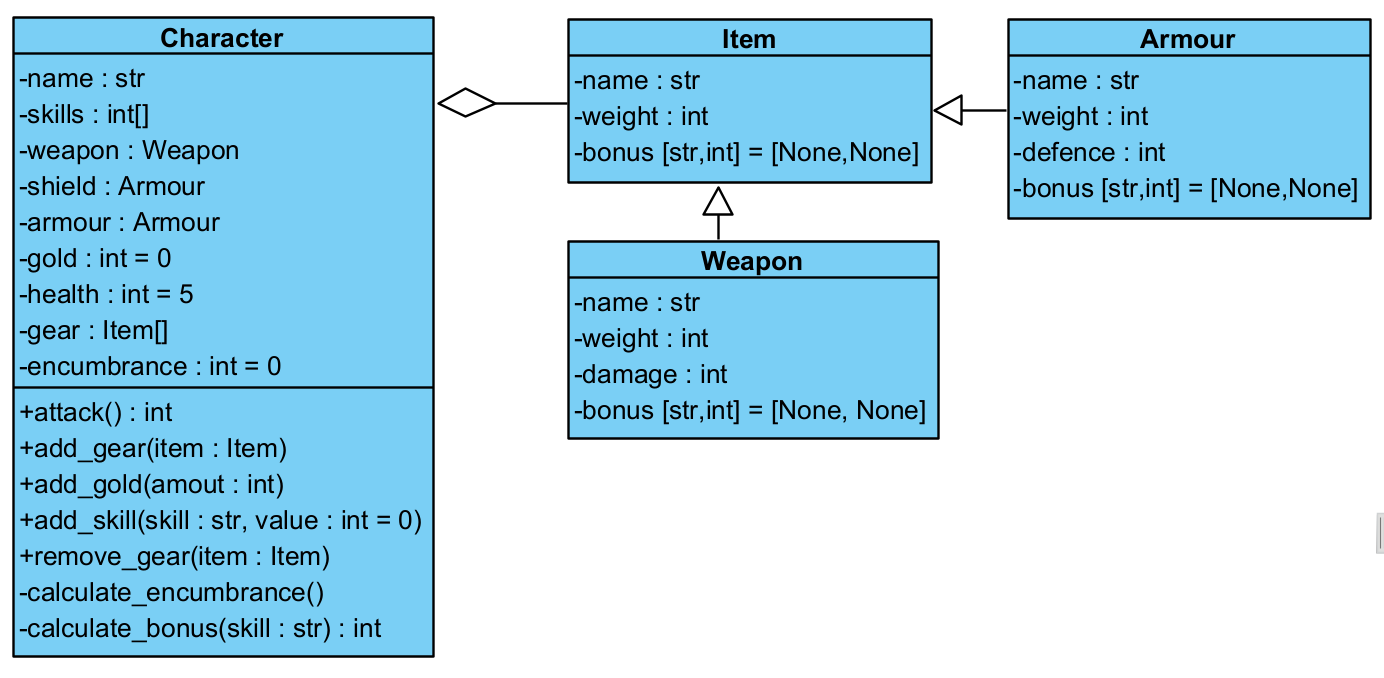
\includegraphics[width=\linewidth]{UML.png}

\end{frame}

\begin{frame}
	\frametitle{Beskrivning av metoder}
	
	\begin{itemize}
		\item \texttt{attack()} ska rulla lika många tärningar med funktionen \texttt{roll\_die} som summan av sin egen färdighet och bonusen från alla föremål  med namnet ''attack''. Funktionen ska returnera summan av alla tärningarna.
		\item \texttt{add\_gear()} ska lägga till ett föremål i listan över \texttt{gear}
		\item \texttt{add\_gold()} ska lägga till talet amount till karaktärens mängd av guld
		\item \texttt{add\_skill()} ska lägga till en färdighet och dess nya värde till ordlistan med färdigheter
		\item \texttt{remove\_gear()} ska plocka bort den första instansen av föremålet man skickar in
		\item \texttt{calculate\_encumbrance()} ska summera alla föremåls vikt och spara i instansvariabeln \texttt{encumbrance}
		\item \texttt{calculate\_bonus()} ska summera all bonus till färdigheten från alla föremål och returnera detta
	\end{itemize}
	
\end{frame}

\end{document}